\documentclass[12pt]{article}
\usepackage[english]{babel}
\usepackage[utf8x]{inputenc}
\usepackage[T1]{fontenc}
\usepackage{listings}
\usepackage{tikz}
\usepackage{/Users/songye03/Desktop/math_tex/style/quiver}
\usepackage{/Users/songye03/Desktop/math_tex/style/scribe}

\begin{document}
Songyu Ye

These are notes from my meeting with Allen on April 12. 
They are interspersed with the toric variety reading group as well as some interesting comments from afterwards.


\section{Combinatorics}

We were thinking about the following rational cone: quadruples $(\lambda,\mu,p_1,p_2)$ where $\lambda,\mu$ are 
dominant weights with $\mu\leq\lambda$ and $p_1,p_2$ are Gelfand-Tsetlin patterns with the same base $\mu$.

\hfill

In particular we are considering this because this is the cone of the affine toric variety to which $\bar{\hat G}$ degenrates.
Recall that $\bar{\hat G}$ is the affine scheme associated to the total coordinate ring of $\bar G$.

\hfill

The suggestion is to begin computer searching and staring at the guys which are not sums. We only have to do this for the projection of the cone onto the $\lambda,\mu$ coordinates. This is related to the fact that we know how to write the patterns as sums of fundamental patterns. Also recall that if the lines which split up the Gelfand-Tsetlin pattern touch, then we get a relation corresponding to the different ways to add together the fundamental patterns ($p_\lambda p_\mu = p_{\lambda\cap \mu} + p_{\lambda\cup \mu}$). These are the relations which generate.

\hfill 

We considered the following example: \begin{center}
    \includegraphics*[scale = .1]{/Users/songye03/Desktop/math_tex/img/B846EC92-9BFA-4E4A-8318-F7784546A319.jpeg}
\end{center}

\section{Reading Group}

We showed that the toric variety associated to a fan is seperated. Recall that this means that the diagonal map $\Delta: X\to X\times X$ is a closed embedding. 

\hfill

\begin{remark}
    One way to think about being seperated is that limits of sequences are unique. This is a good way to think about it because it is a analagous to the Hausdorff property for topological spaces. The point is that for any DVR $R$, $\Spec R$ has two points, corresponding to the two prime ideals $0$ and those guys with valuation $\geq 1$. Let $F$ denote the field of fractions of $R$. $\Spec F$ consists of a single point, the generic point. Then there is the following 
    valuative criterion for being seperated. 
        
    \begin{theorem}
        $X$ is seperated if and only if for any DVR $R$ and any morphism $\Spec R\to X$ there is at most one way to fill in the diagram.

        \begin{center}
            \begin{tikzcd}
                \Spec F \arrow[r] \arrow[d] & X \\
                \Spec R \arrow[ur, dashed]
            \end{tikzcd}
        \end{center}
    \end{theorem}

    The point is that the generic point of $\Spec F$ represents a neighborhood of the origin with the origin actually removed, and the extension is about filling in the origin. An example of $R$ are the power series ring $k[[t]]$ and then the 
    corresponding field of fractions is $k((t))$.
\end{remark}

\hfill

The point of the proof is that the fan tells us how to assemble affine pieces together to get the toric variety, and the pieces are glued together in a nice enough way. In particular it is not necessarily true that any scheme which is covered by affine varieties is seperated. The line with two origins is an example of this (a nice way to see that it is not seperated is by using the valuative criterion).

\hfill

In particular one ends up showing the following. 

\begin{lemma}
    The map $U_\sigma \to U_{\tau_1}\times U_{\tau_2}$ is a closed embedding.
\end{lemma}

This is very closely related to the following. A scheme $X$ is quasiseperated if and only if for every pair of affine opens $U,V \subset X$ the intersection is a finite union of affine opens. This is a weaker condition than being seperated. The point is that if $\Delta: X\to X\times X$ is quasicompact, then the preimage of an affine open $U\times V \subset X\times X$ is necessarily quasicompact, and then one observes that the preimage is precisely $U\cap V$.

\hfill

\begin{theorem}
    $f$ is seperated if and only if for every pair of affine opens $U,V\subset X$ the intersection $U\cap V$ is affine and the ring map $O_X(U)\otimes O_X(V)\to O_X(U\cap V)$ is surjective.
\end{theorem}

\hfill

The statement about rings reflects the fact that a closed embeddings locally look like ring surjections. Clearly these characterizations show us that seperated implies quasiseparated. 

\hfill

Finally I think it is enough to show the lemma because the property of being a closed embedding is local on the target.
\section{Cartier divisors on toric varieties}

There is a very well known example the ruling by two lines on the quadric cone is not Cartier. This can be generalized by 
a complete characterization of all Cartier divisors on any given toric variety. However we can try to explain things 
in this particular example. We start with the line bundle $O(2)$ on $\P^1$. The polytope looks like an interval
with 3 lattice points. We are thinking about the cone over $\P^1$ so we cone the polytope.

\begin{center}
    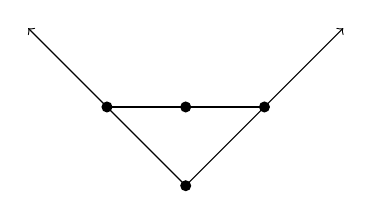
\begin{tikzpicture}

    % Draw lattice points
    \foreach \x in {0,1,2} {
        \fill (\x,0) circle (2pt);
    }
    
    % Draw interval
    \draw (0,0) -- (2,0);
    \fill (1,-1) circle (2pt);
    \draw[->] (1,-1) -- (-1,1);
    \draw[->] (1,-1) -- (3,1);
    \end{tikzpicture}
\end{center}

[Note that these lattice points correspond to the terms $x^2,xy,y^2$ and $x,y$ are not drawn in.]

There is a corresponding picture on the lattice points of $\C^2$ where we only take the black squares on the checkerboard.
This is a consequence of taking the GIT quotient $\C[x,y]^{\Z/2}$ where $\Z/2$ acts by $(x,y)\mapsto (-x,-y)$. Notice that the 
invariant ring looks like $\C[x^2,xy,y^2] \subset \C[x,y]$ which is precisely the coordinate ring of the cone over $\P^1$. Then the ruling on the cone is cut out by for example $y = 0$ which looks like quotienting out by the ideal $\ideal{xy,y^2}$. This is 
not principal so therefore the ruling is not Cartier.

\hfill

Note that $2D$ is indeed Cartier. This is because now we are thinking about the vanishing of $y^2$ and this corresponds to the $y^2$ term vanishing and the $xy$ squares to zero. This means we are thinking about the ring $\C[x,u]/\ideal{u^2}$ which corresponds to a principal ideal and is therefore Cartier. The corresponding subscheme looks like a doubled point times a line.


\section{Computing sheaf cohomology as lattice points}

It is a general thing for spaces with a torus action that the higher cohomology groups can be computed as lattice points inside some corresponding polytope. The lattice points represent the weights which appear in the cohomology when one decomposes as a representation. For toric varieties, it is the case that each of these weights will just appear with multiplicity 1.

\begin{center}
    \includegraphics*[scale = .1]{/Users/songye03/Desktop/math_tex/img/474A7601-E3E1-42C0-8776-4DEA18642100.jpeg}
\end{center}
\red{"principal of inclusion exclusion"}

\subsection{References}
The corresponding papers to read are: 
\begin{itemize}
    \item Karshon-Tolman (Symplectic)
    \item M. Braverman
    \item Siye Wu Equivaraint Holomorphic Morse Inequalities
    \item Constantin Teleman
\end{itemize}


\section{Equivariant homology of infinite dimensional Lie groups}
This is a followup to the remark that Allen made a long time ago, the note from my phone reads:

\begin{remark}
    "splitting root systems in half B- orbits and B orbits correspond to cohomology slice the other way to get some infinite codimension and dimension"
\end{remark}
\red{really wise stuff}. Here are some things that one can say.
\subsection{Infinite dimensional lie groups}
In the finite dimensional story, picking a Borel amounts to picking half the root system and then one discovers that all of the Borels are conjugate under the action of the Weyl group. Now consider $A_3$ root system crossed with $\Z$. This root system is infinite and there are a couple of different ways to slice it. One way is to take all the guys left of $0$ in $\Z$. As it turns out, if this is $B$, then all of the $B$ orbits in $G/B$ will be finite dimensional and all of the $B-$ orbits will be finite codimensional, and all of the choices of this type up to finiteness are Weyl conjugate.

\hfill 

However another way to slice is along the $\Z$ axis and in this way we obtain a $B$ for which the $B$ orbits are infinite dimensional and the $B-$ orbits are infinite codimensional. This is a different way to slice the root system and the corresponding $B$ is not Weyl conjugate to the previous $B$.

\subsection{Equivariant homology}
In the $T$-equivariant homology of the flag variety, we can do something similar to equivariant cohomology. As it turns out, equivariant homology almost forms a $H_*^T$ module, it does after formally inverting things and passing to the quotient field. 

\hfill

For example consider the following $\P^1$ inside the flag variety of $\SL_3(\C)$.

\begin{center}
    \includegraphics*[scale = .09, angle = -90]{/Users/songye03/Desktop/math_tex/img/A739D5D8-CE62-4C70-82B0-D1A0CC4990AA.jpeg}
\end{center}

The annotations denote the expansion of the $\P^1$ in terms of classes of the $T$ fixed points. Note that this is good because now the pushforward to a point of that $\P^1$ is indeed zero, as it should be geometrically.

\subsection{Question}
I guess the point of what one could try to work on in this setting is making sense of what should the class of a $B$-orbit should be. We know that in the ordinary flag variety, the $B$ orbits form a basis for the cohomology/homology. We can also think of cup and cap products. 

\subsection{References}
\begin{itemize}
    \item Semi-infinite combinatorics in representation theory (Lanini)
\end{itemize}

\end{document}

